% !TeX root = ../thesis.tex

\chapter{Modell}
\label{sec:modell}
Dieses Kapitel befasst sich mit der Herangehensweise an die praktische Umsetzung des Modells zur Vorführung seiner Funktion. In den vorausgegangenen Kapiteln wurden jegliche Grundlagen und theoretische Veranschaulichungen vertieft, welche notwendig sind, um nun anwendungsorientiert in einem gegenständlichen elektrischen Sender manifestiert zu werden. Daher wurde zur Erstellung eines Modells zunächst eine \gls{acr:LT}-Spice Simulaion des analogen Signalverarbeitungsschaltkreises erstellt. Zudem beschäftigt sich dieses Kapitel mit der Planung und Erstellung eines Platinenlayouts zur Komprimierung der Realisierungsgröße des Schaltkreises. Im Anschluss wird der Aufbau eines Gehäuses thematisiert, welches zur Unterbringung aller physikalischer Komponenten dienen soll.

\section{Simulation in LT-Spice}
\label{sec:simlt}

Zunächst wurde das vorausgegangene theoretische Wissen mit einer LT-Spice Simulation überprüft. So konnten eventuelle Fehler bei der Dimensionierung ermittelt und verbessert werden. Hierbei wurden die analogen Schaltungsteile, welche in Kapitel~\ref{sec:Signalverarbeitung} näher ausgeführt wurden, zusammengefügt. Zudem wurde der DC/DC-Wandler mit in die Schaltung eingebunden, um die \gls{acr:OP}s mit einer negativen Spannung zu versorgen. Die Versorgungsspannungen wurden durch Tiefpassfilter an den \gls{acr:OP}s erweitert, um hier hochfrequente Störungen zu filtern. Des Weiteren wurde ein \gls{acr:DC}-Abblock-Kondensator zwischen Soundkarte und der ersten Stufe der analogen Signalverarbeitung vorgesehen, um der Schaltung nur das reine \gls{acr:AC}-Signal zuzuführen. Abbildung~\ref{fig:spice} illustriert die simulierte Schaltung in der Darstellung des LT-Spice Softwarefensters.

\begin{figure}[H]
	\centering
	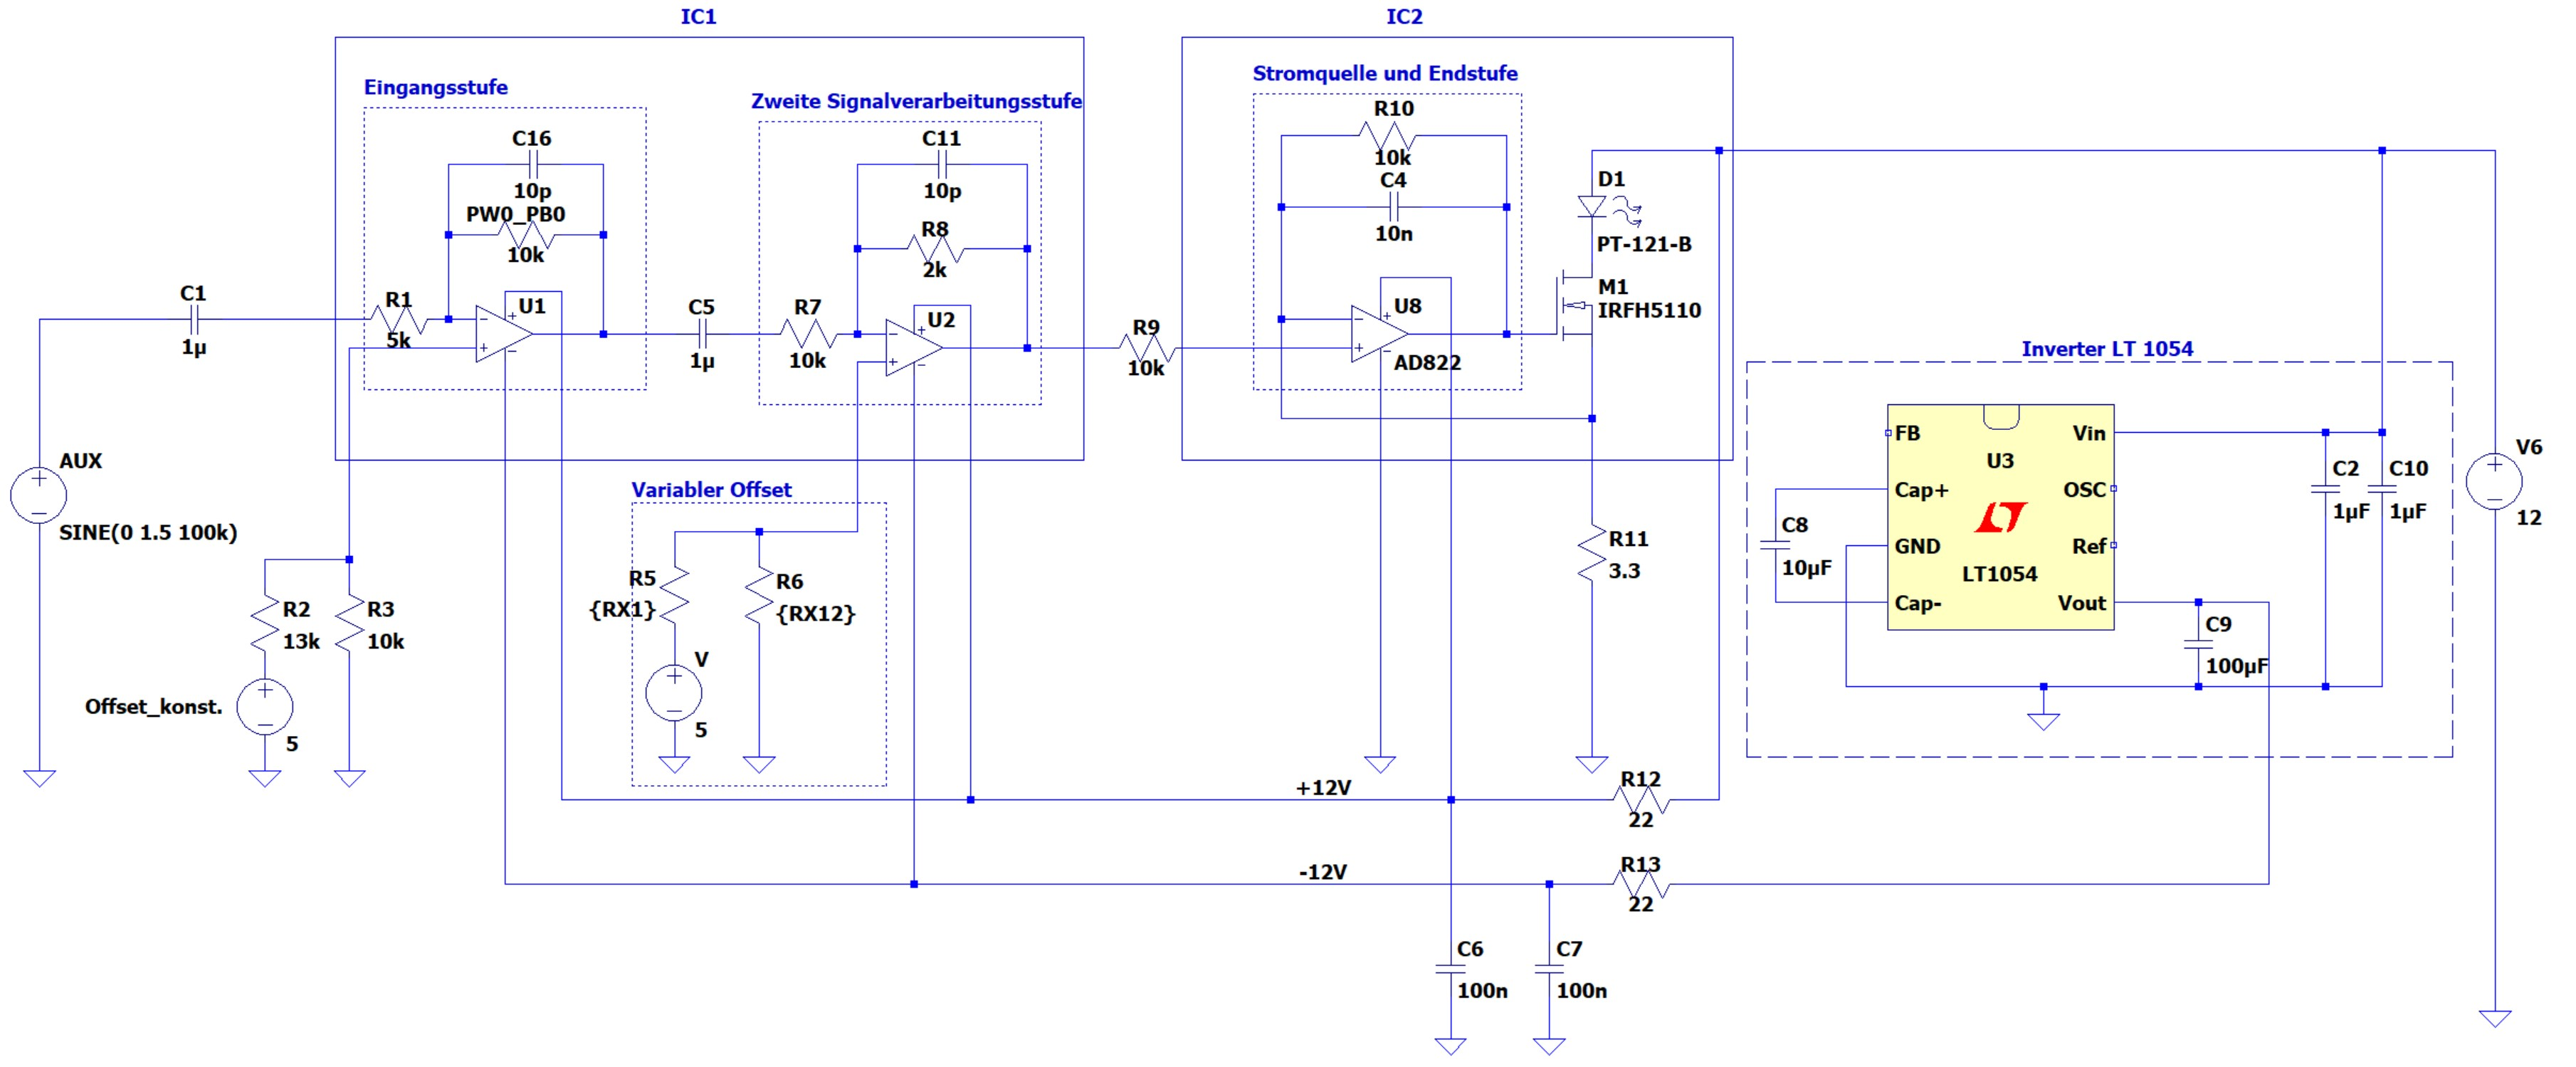
\includegraphics[width = 0.9 \textwidth ]{spice.jpg}
	\caption[LT-Spice Simulation der Signalverarbeitung]{LT-Spice Simulation der Signalverarbeitung} \gls{online:Eigen}
	\label{fig:spice}
\end{figure}

\section{Platinenlayout in \gls{acr:EAGLE}}
\label{sec:platineeagle}

Bei dem Entwurf des Platinenlayouts für den Sender wurde ein besonderes Augenmerk auf die Trennung von Signal- und Leistungspfaden gelegt, um mögliche Interferenzen der beiden Pfade zu minimieren.

\begin{figure}[H]
	\centering
	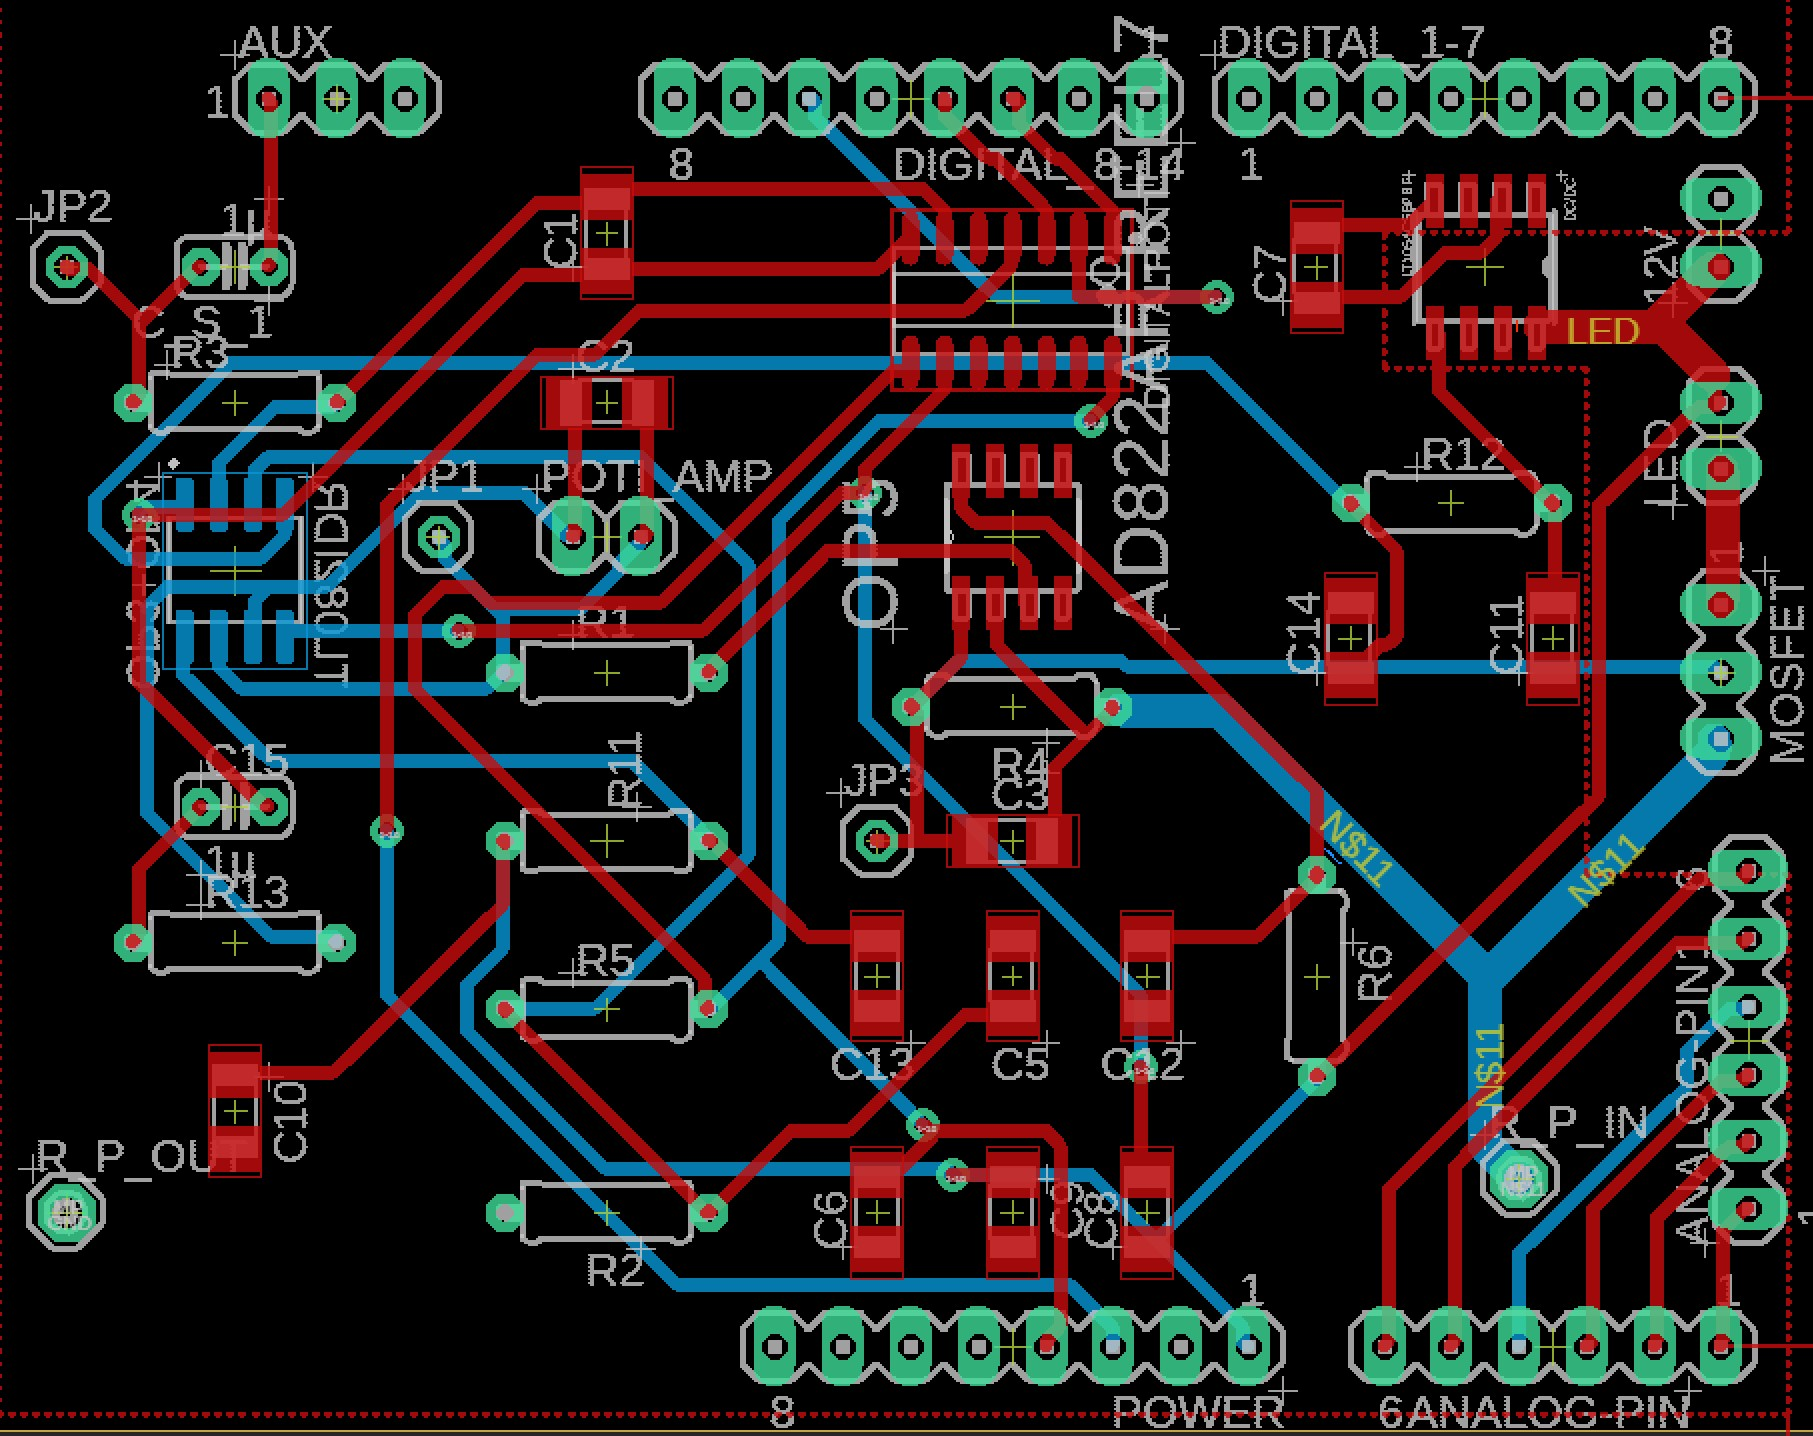
\includegraphics[width =1 \textwidth ]{eagle.jpg}
	\caption[\gls{acr:EAGLE} Auszug der Platine]{\gls{acr:EAGLE} Auszug der Platine} \gls{online:Eigen}
	\label{fig:eagle}
\end{figure}

Im unteren Bereich der Platine befindet sich der Leistungswiderstand, welcher sich von $R-P-IN$ zu $R-P-OUT$ erstreckt. Zuzüglich befinden sich der DC/DC Spannungswandler, \gls{acr:LED} und \gls{acr:MOSFET}, die signifikanten Bauteile der Stromquelle, auf der rechten Seite der Platine und somit möglichst weit vom Signalverarbeitungspfad entfernt. In der Schaltung fließen teilweise Ströme von bis zu 1,42A. Da es bei solch hohen Strömen zu Problemen mit der \gls{acr:EMV} kommen kann, wurde der Signalweg linksseitig auf der Platine positioniert. Außerdem wurden die Leiterbahnen im Leistungspfad besonders breit ausgelegt, da hier große Ströme fließen. Genaue Informationen über die Dimensionierung der Leiterbahnen und Abstände sind in Tabelle~\ref{tab:leiterbahnen} zu finden. Diese sind signifikant für die Dimensionierung des Platinenlayouts. Hier werden die verschieden Leiterbahnbreiten und Leiterbahnabstände dargestellt, welche für ein funktionierendes Platinenlayout unabdingbar sind.

\begin{table}[htb]
	\begin{center}
		\begin{tabular}[h]{cccc}	
			\toprule
			Spannung [V] & Max. Strombelastung [A]& Leiterbahnbreite [mil] & Leiterbahnabstand[mil] \\
			\midrule
			5 & 0.6&6 & 8 \\
			10 & 0.8&8 & 13 \\
			30 & 2.0&20& 30\\
			150 &2.7&30 & 50 \\
			230& 3.5&50 & 100 \\
			\bottomrule
		\end{tabular}
		\caption{Richtlinien zu Leiterbahnbreite und Leiterbahnabständen}\gls{online:eagleleit}
		\label{tab:leiterbahnen}
	\end{center}
\end{table}


Hinzu wurden auf der Platine für die Operationsverstärker, das Digitalpotentiometer und den DC/DC Spannungswandler IC-Sockel aufgelötet. Das ermöglicht den schnellen Austausch von defekten Bauteilen, sowie bei der Fertigung der Platine, möglichen thermischen Beschädigungen vorzubeugen. Um die Bauform der Platine möglichst kompakt zu halten, wurde iene Dual-Layer Platine entworfen. Hierbei werden sowohl auf der Vorder-, als auch auf der Rückseite Leiterbahnen vorgesehen und ausgefräst. Die Leiterbahnen auf der Rückseite sind in Abbildung~\ref{fig:eagle} durch die blauen Leiterbahnen dargestellt. Des Weiteren wurden im Signalverarbeitungspfad nach jeder Stufe Messpunkte vorgesehen, um die Fehlersuche zu erleichtern und nachträglich einzelne Funktionsprüfungen durchzuführen. Außerdem ist zu beachten, dass die Bauteile im Leistungspfad durch den hohen Stromfluss eine hohe thermische Abgabe an Energie verzeichnen müssen. Um die dadurch entstehende Wärme besser abzuführen, wurden Kühlkörper vorgesehen. Wie diese berechnet und dimensioniert werden, wird in Kapitel~\ref{subsub:thermo} näher erläutert. Um die Schaltung störresistenter zu gestalten, wurden die gegebenen freien Flächen auf beiden Seiten der Platine mit dem Massepotential ausgefüllt. 

\newpage
\section{Planung und Aufbau des Gehäuses}
\label{sec:geh}

In den vorausgegangenen Unterkapiteln wurden sowohl die Schaltungsteile, als auch die Wichtigkeit einer ausreichenden Kühlung der Bauteile verdeutlicht. Nun galt es, all diese Hardwarekomponenten zu einem großen Ganzen zusammen zu fassen, um somit ein in sich beständiges System zu schaffen. Demnach wurde für die kompakte und ansehnliche Unterbringung aller Hardwarekomponenten ein 3D-Druck-Gehäuse konstruiert. Hierbei wurde so platzsparend wie möglich gearbeitet. Aussparungen für die Datenschnittstelle, Audiobuchse und Spannungsversorgung wurden so angeordnet, dass diese jederzeit zugänglich sind. Zudem wurden drei Seiten mit ausreichend Lüftungsschlitzen bestückt, um der Wärmeentwicklung im Gehäuse entgegen zu wirken. Des weiteren wurde eine Aussparung für einen mit $12V$ betriebenen Lüfter vorgesehen. Dieser soll zusätzlich für einen Luftstrom im inneren des Gehäuses sorgen und somit eine bessere Kühlung gewährleisten. Abbildung~\ref{fig:3dbottom1} und Abbildung~\ref{fig:3dbottom2} veranschaulichen die 3D-Ansicht dieses Gehäuses.

\begin{figure}[H]
	\centering
	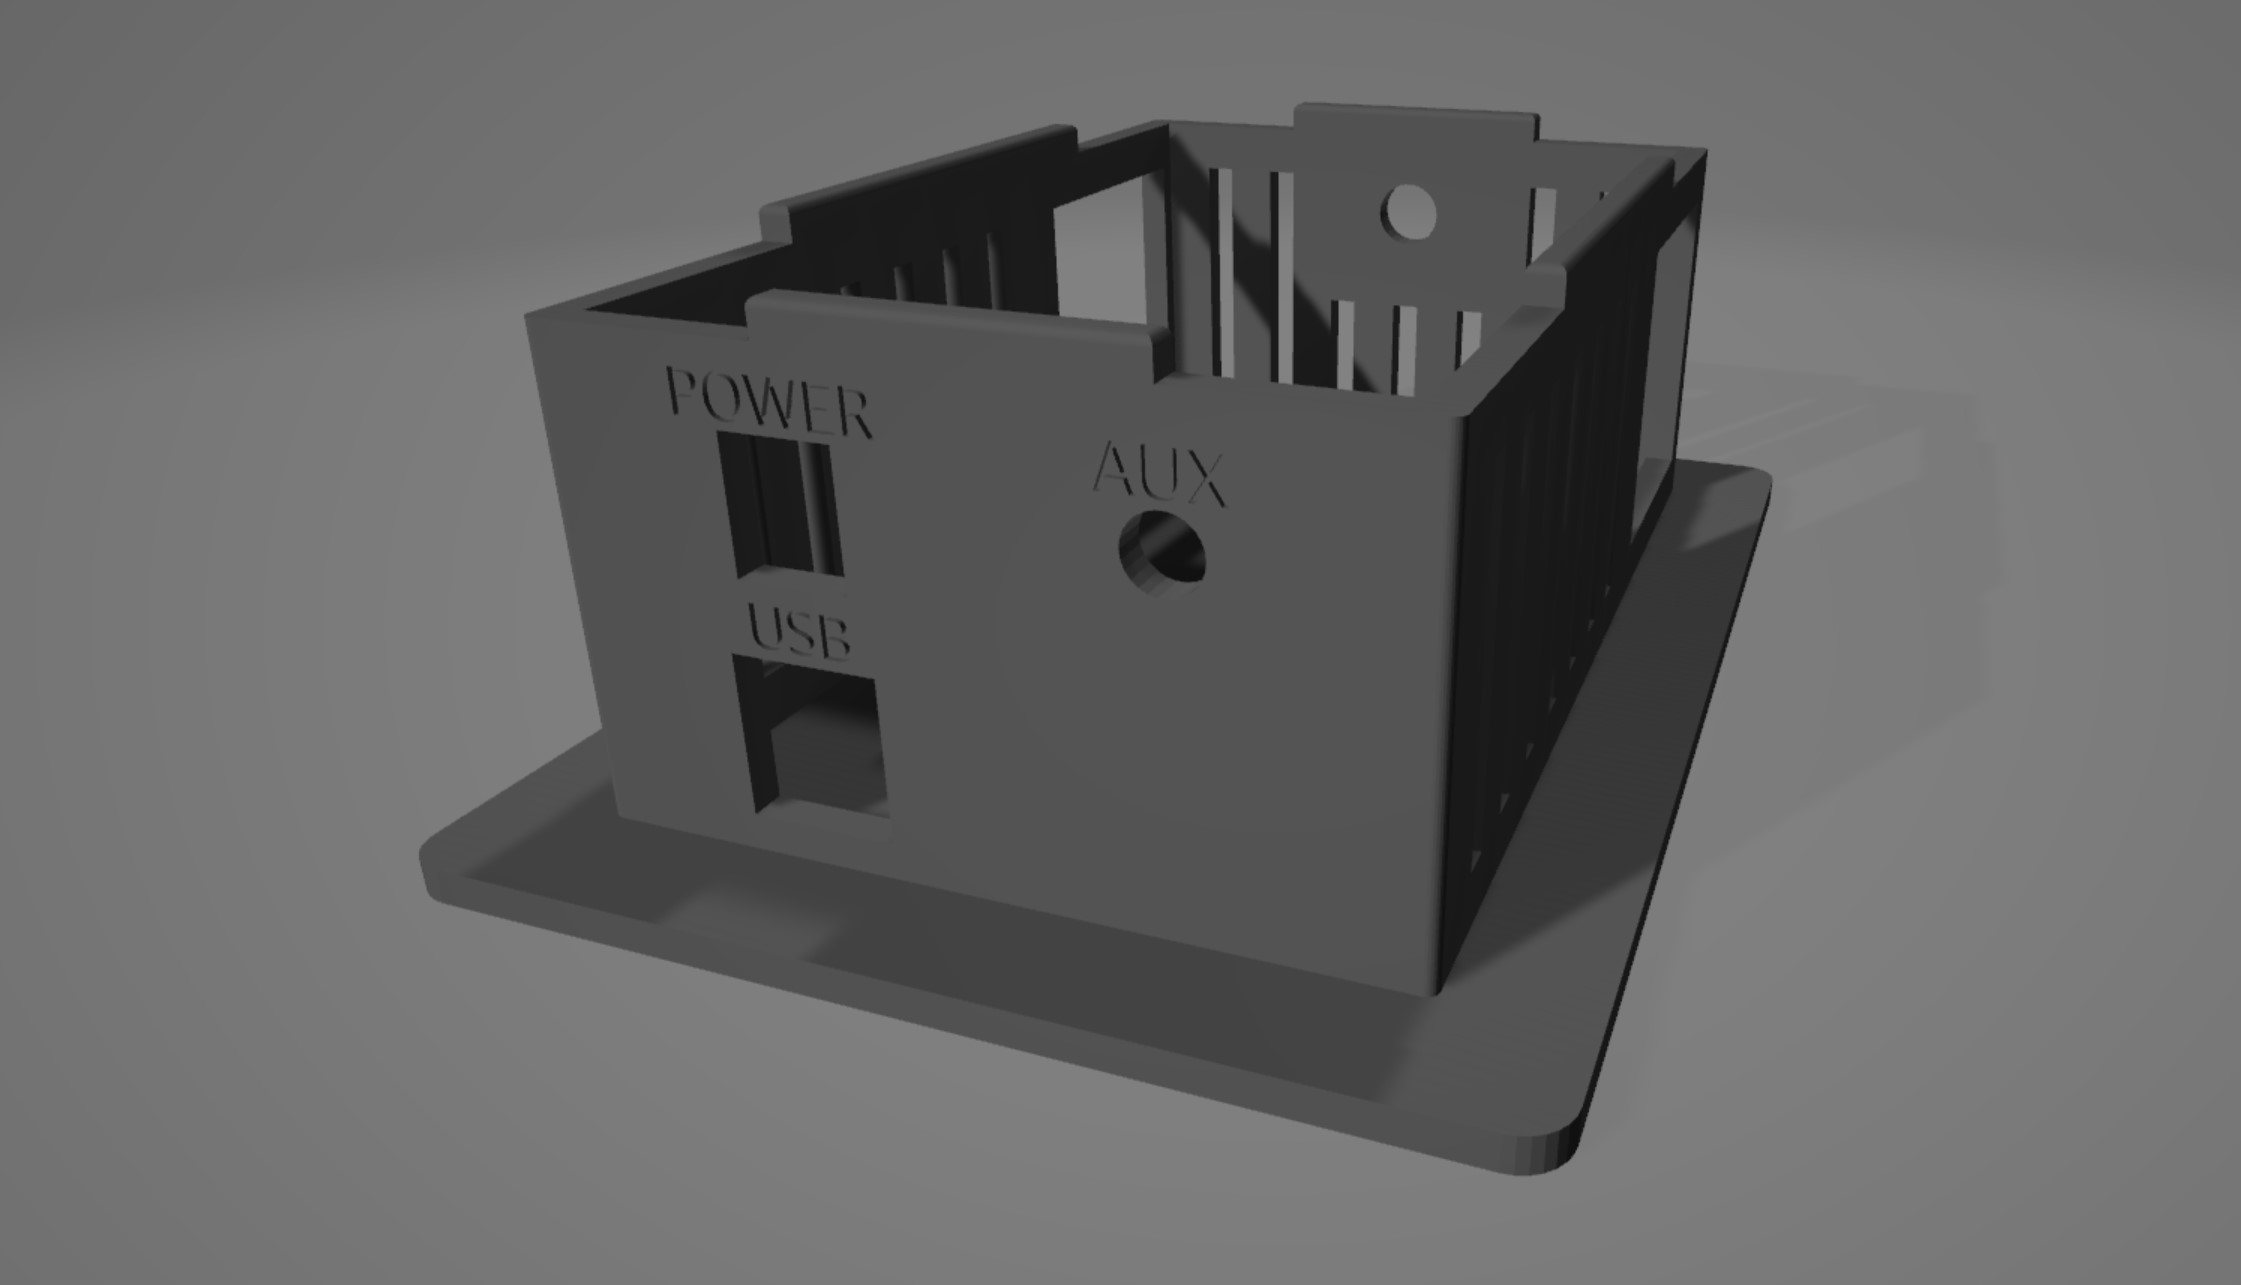
\includegraphics[width =0.9 \textwidth ]{3dbottom1.jpg}
	\caption[Boden des 3D-Drucks]{Boden des 3D-Drucks} \gls{online:Eigen}
	\label{fig:3dbottom1}
\end{figure}

Der Arduino wird am Boden des Gehäuses fixiert und bietet die Basis des analogen Schaltungsteils.
Da sich Leistungswiderstand, Transistor und Leuchtdiode im Betrieb erhitzen, wurden die zugehörigen Kühlkörper nah am Lüfter montiert.

\begin{figure}[H]
	\centering
	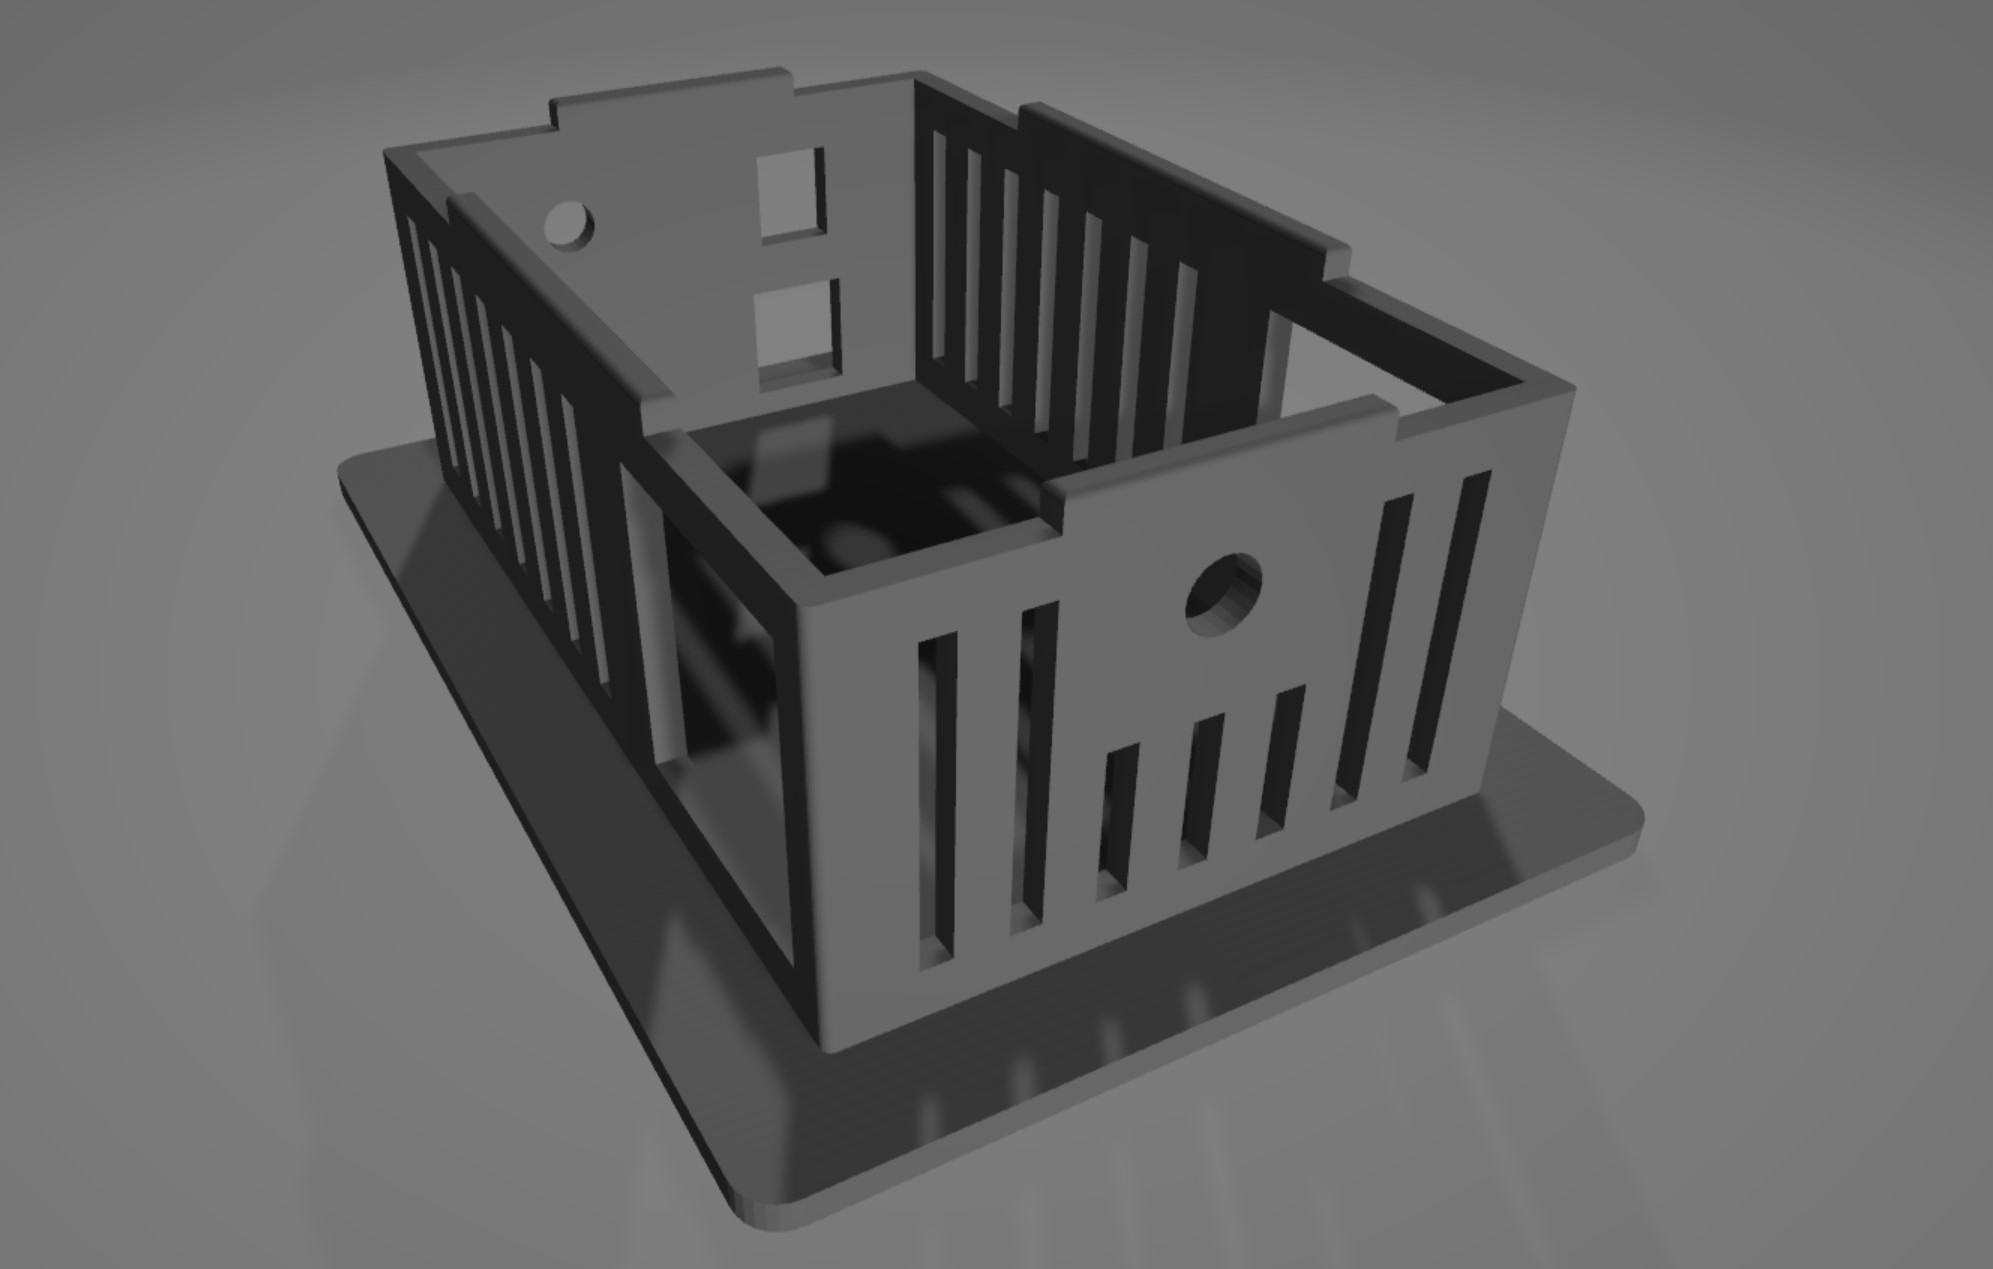
\includegraphics[width =0.9 \textwidth ]{3dbottom2.jpg}
	\caption[Boden des 3D-Drucks]{Boden des 3D-Drucks} \gls{online:Eigen}
	\label{fig:3dbottom2}
\end{figure}

Zusätzlich wurde im Deckel eine Öffnung für den Einbau eines \gls{acr:LCD} vorgesehen, um dort Statusinformationen des Senders visuell auszugeben. Für das Zu- und das Abschalten der Spannungsversorgung wurde nachträglich im Deckel noch ein Schalter verbaut.

\begin{figure}[H]
	\centering
	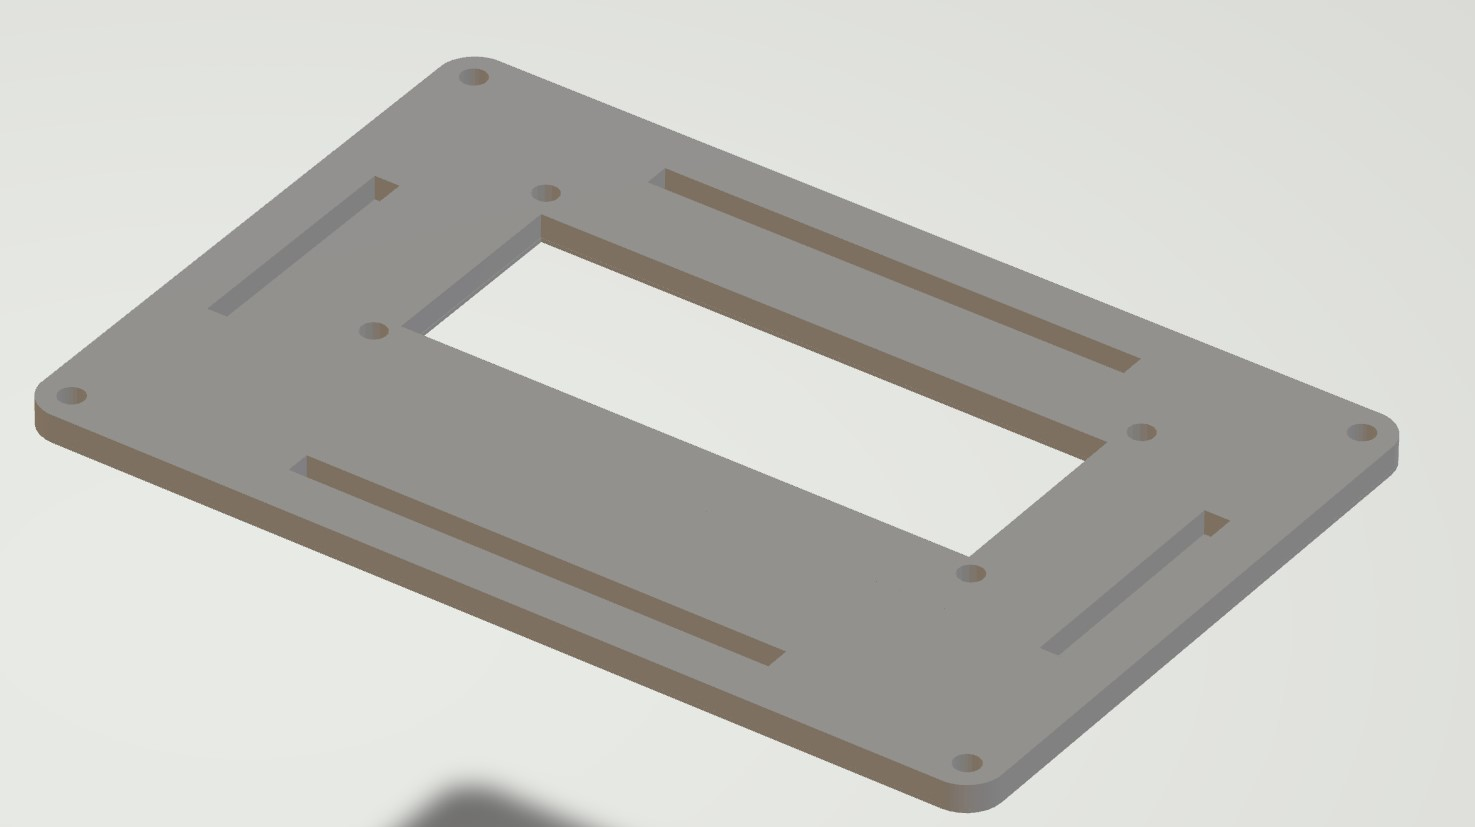
\includegraphics[width =0.9 \textwidth ]{3dtop.jpg}
	\caption[Deckel des 3D-Drucks]{Deckel des 3D-Drucks} \gls{online:Eigen}
	\label{fig:3dtop}
\end{figure}





